\section{Plano de trabalho}

Tendo em conta a dimensão da aplicação, foi criado um plano de trabalho onde se mapearam as tarefas
de desenvolvimento no tempo de forma contínua, tornando assim possível adaptar um ritmo de trabalho
consistente com os prazos de entrega de cada fase e então cumprir as metas do projeto.

Nesse sentido dividiu-se o projeto em três fases, sendo elas o \textbf{planeamento e análise de requisitos}, o
\textbf{desenvolvimento} e a \textbf{documentação}.

No que diz respeito à fase de planeamento e análise de requisitos, esta fase engloba todo o levantamento 
de funcionalidades assim como todo o planeamento e estruturação do projeto 
nomeadamente, criação do modelo de domínio, diagrama de classes, modelação do repositório de dados,
análise da concorrência, plano de trabalho, plano tecnológico, casos de estudo, arquitetura do sistema, etc.

Para esta fase de planeamento, análise e modelação foi criado um plano de um mês onde todas as tarefas 
teriam de estar concluídas. Na Figura \ref{fig: workplan1} é possível ver um diagrama de Gantt com
o planeamento inicial.

\begin{figure}[H] 
  \centering
  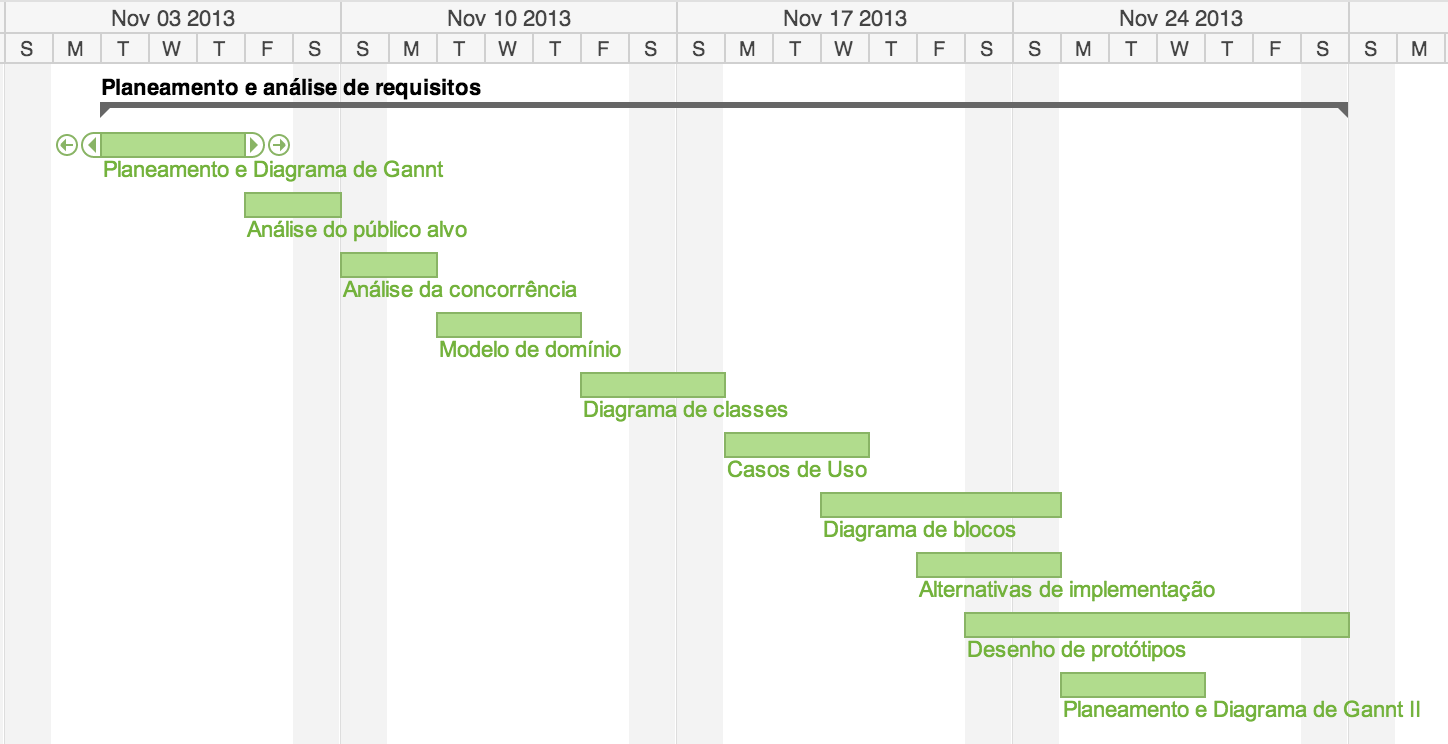
\includegraphics[width=1\textwidth]{images/plano_de_trabalho/gannt_1.png}
  \caption{Diagrama de Gantt para o planeamento e análise de requisitos}
  \label{fig: workplan1}
\end{figure}

De seguida, prosseguindo para o planeamento da fase de desenvolvimento após 
analisar as funcionalidades e modelar o sistema  é altura de começar a 
prototipar a aplicação e começar a iterar sobre as funcionalidades a 
implementar. Neste sentido englobaram-se aqui tarefas como prototipagem em HTML, 
criação de migrações na modelação da base dados, modelação das entidades a 
representar (modelos) na forma da arquitetura MVC seguindo-se a implementação dos 
controladores e visões, tendo como base as funcionalidades a desenvolver para o 
sistema. Nesta fase pretende-se tornar a aplicação capaz de suportar os seus 
utilizadores (não registados, docentes e alunos) das tarefas de gestão de UCs, 
projetos, grupos e submissões, assim como consulta e disponibilização de 
projetos. No que diz respeito à metodologia de desenvolvimento seguir-se-ão 
os métodos e princípios de desenvolvimento de software \textit{Agile}. Posto isto, 
far-se-á um desenvolvimento cíclico e iterativo focado em cada grupo de 
funcionalidades, desenvolvendo-as, testando-as e validando-as. Caso seja 
necessário fazer novas iterações sobre um grupo de funcionalidades, basta 
repetir o ciclo até que seja possível validar o que foi desenvolvido e de seguida inicia-se 
um novo ciclo de desenvolvimento para o grupo de funcionalidades seguinte.

Desta forma é possível uma rápida adaptação a mudanças e ajustes sem ter que verificar e 
revalidar todo o planeamento inicial do projeto e ainda assim atingir as metas 
definidas.

Faça-se notar que em cada ciclo de desenvolvimento para além da implementação,
 serão feitos testes de usabilidade e funcionalidade, dessa forma é possível garantir que em cada estado do 
desenvolvimento, todas as funcionalidades implementadas encontram-se o mais perto 
do idealizado possível.
Durante cada ciclo de desenvolvimento também faremos a integração da 
documentação relativa ao grupo de funcionalidades que estão a ser implementadas.
É possível ver nas Figuras \ref{fig: workplan2}, \ref{fig: workplan3}, \ref{fig: workplan4} 
os diagramas de Gantt com o planeamento respetivo à fase de desenvolvimento.

\begin{figure}[H] 
  \centering
  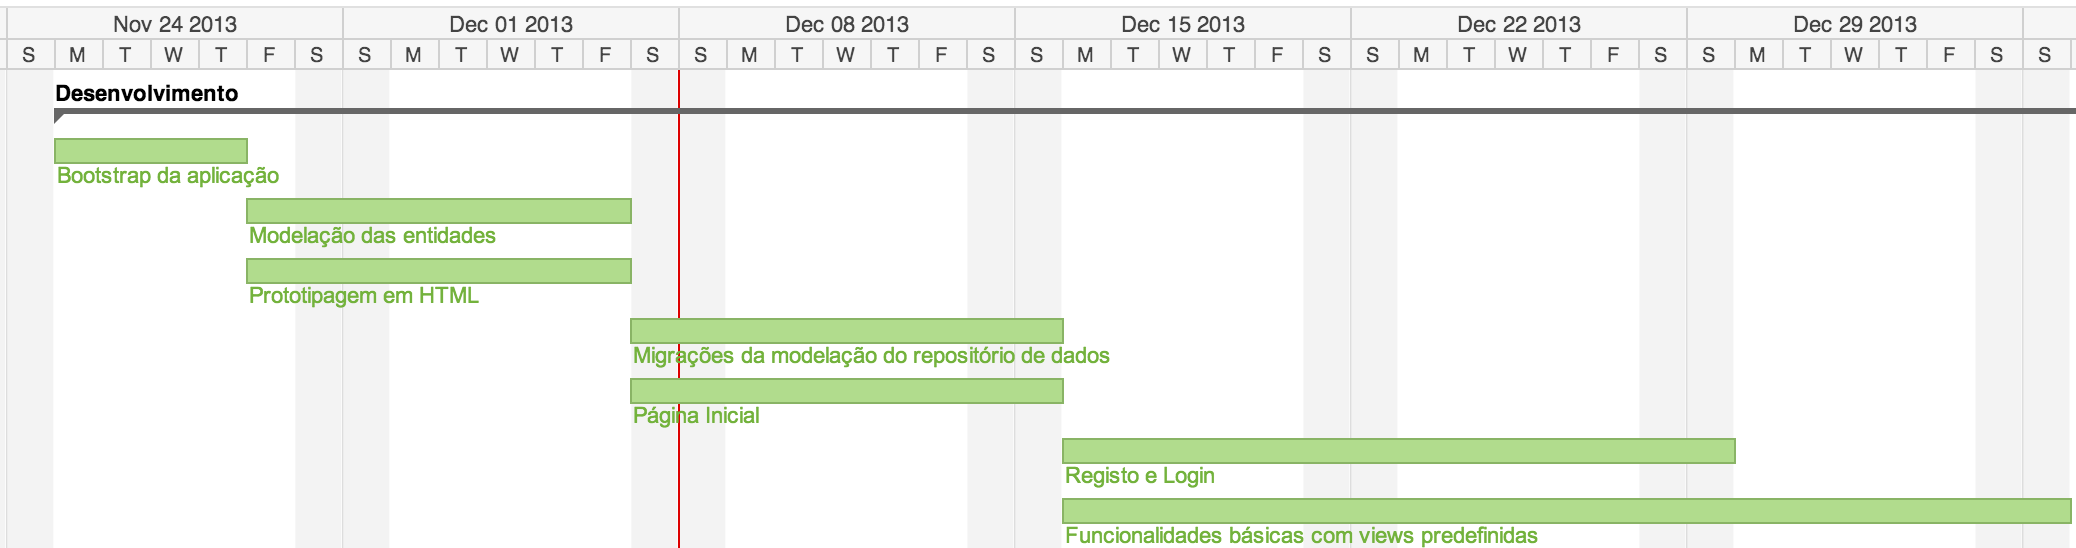
\includegraphics[width=1\textwidth]{images/plano_de_trabalho/gannt_2.png}
  \caption{Diagrama de Gantt para o desenvolvimento I}
  \label{fig: workplan2}
\end{figure}

\begin{figure}[H] 
  \centering
  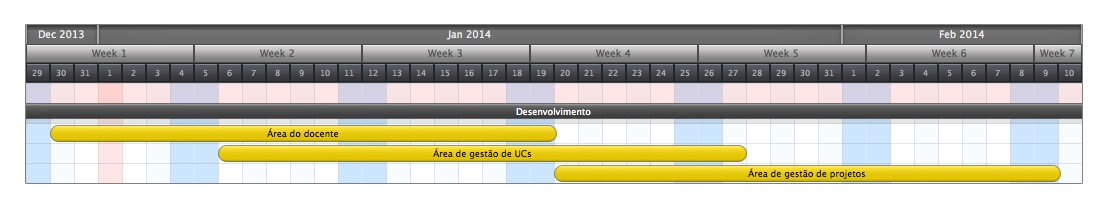
\includegraphics[width=1\textwidth]{images/plano_de_trabalho/gannt_3.png}
  \caption{Diagrama de Gantt para o desenvolvimento II}
  \label{fig: workplan3}
\end{figure}

\begin{figure}[H] 
  \centering
  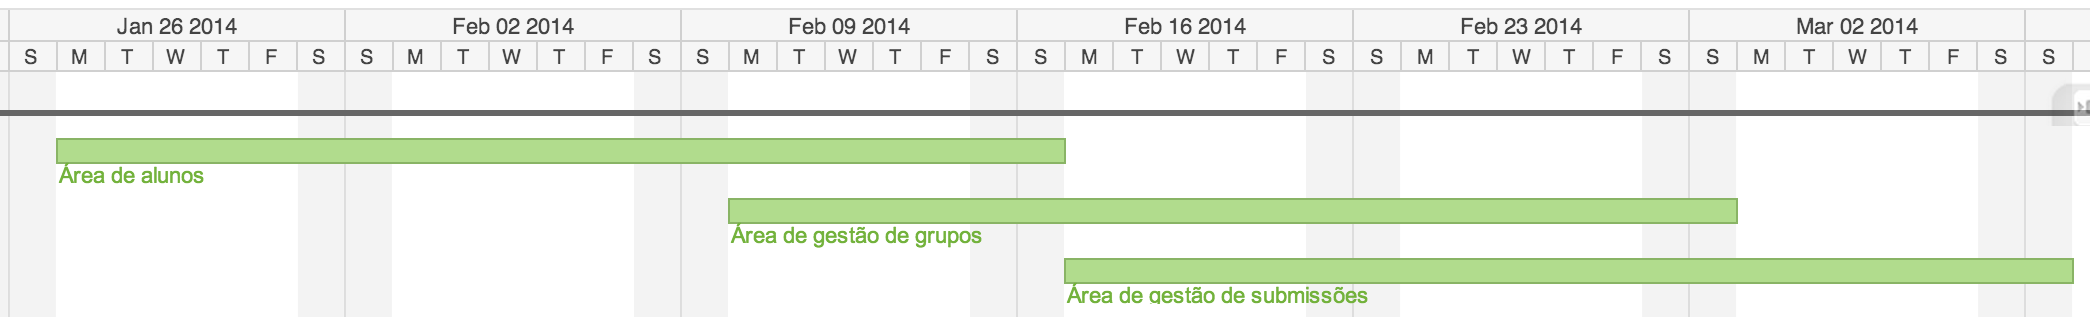
\includegraphics[width=1\textwidth]{images/plano_de_trabalho/gannt_4.png}
  \caption{Diagrama de Gantt para o desenvolvimento III}
  \label{fig: workplan4}
\end{figure}

Por fim, terminámos com a fase de documentação onde será feita toda a descrição 
do sistema desenvolvido em termos de funcionalidades e implementação de forma a 
possibilitar a consulta tanto aos interessados em utilizar a aplicação bem como 
de forma a suportar a possível necessidade de manutenção da aplicação. Desta 
forma qualquer um pode entender todo o sistema na sua plenitude através da 
documentação criada. As tarefas desta fase serão distribuídas pelos ciclos de 
desenvolvimento falados acima, em que cada fase de documentação será empregue no 
mesmo ciclo de desenvolvimento das funcionalidades respetivas.

O diagrama de Gantt completo encontra-se representado em Anexo na Figura \ref{fig: 
workplan0}.

\newpage
